% !TEX root = sprints.tex
\noindent \large{\textbf{Summary}}\\
\normalsize Team Expeditus was unfortunately unable to complete the tasks for sprint 5, but the team was able to make measurable progress towards the goals. After deciding not to pursue simulation, the team members began to focus on message passing and offboard control between the flight controller and the Odroid. After multiple issues with multiple approaches to the AR tag tracking, the team was able to successfully get the AR Track Alvar library up and running.
\vspace{5mm}
\\
\noindent \Large{\textbf{Team Work}}
\normalsize
\begin{itemize}
\item \textbf{Jonathan Dixon:} Worked on AR tracking.
\item \textbf{Dylan Geyer:} Worked on AR tracking.
\item \textbf{Christopher Smith:} Worked on message passing and offboard control. 
\item \textbf{Steven Huerta:} Worked on AR tracking. 
\end{itemize}

\vspace{5mm}
\noindent \Large{\textbf{Uncompleted Tasks}}\\
\vspace{2mm}\\
\noindent \large{\textbf{As an owner, I want the UAV to autonomously land on the landing pad without damaging the craft}}
\normalsize
\begin{itemize}
\item \textbf{Visual Tracking by use of non-ROS version of AR tracker}\\
The team was able to successfully download, install, and run a non-ROS version of ALVAR to track AR Tags. The GUI elements of the AR Tracking program were removed and replaced by printing the quaternian and translation data of the AR Tag to the terminal.
The team decided not to pursue this any further since we were able to get the AR Track Alvar ROS package working which will save us the time of creating our own ROS wrapper around alvar.

\item \textbf{Visual Tracking by use of ROS version of AR tracker}\\
$AR_TRACK_ALVAR$ is a package in ROS that provides AR tracking. The advantage of using this tool, is that the tracking tool will evaluate the tag, the tag 
\item \textbf{Offboard Local Control of UAV}\\
Though not completed, progress was made on modifying our implementation of the landing algorithm to only include the AR tag tracking. The tracking tool (fig.~\ref{fig:artracker}) that we have successfully tested will provide us with distance information necessary to correctly judge the distance from our landing target, as well as calculate a safe rate of descent.

\begin{figure}[h]
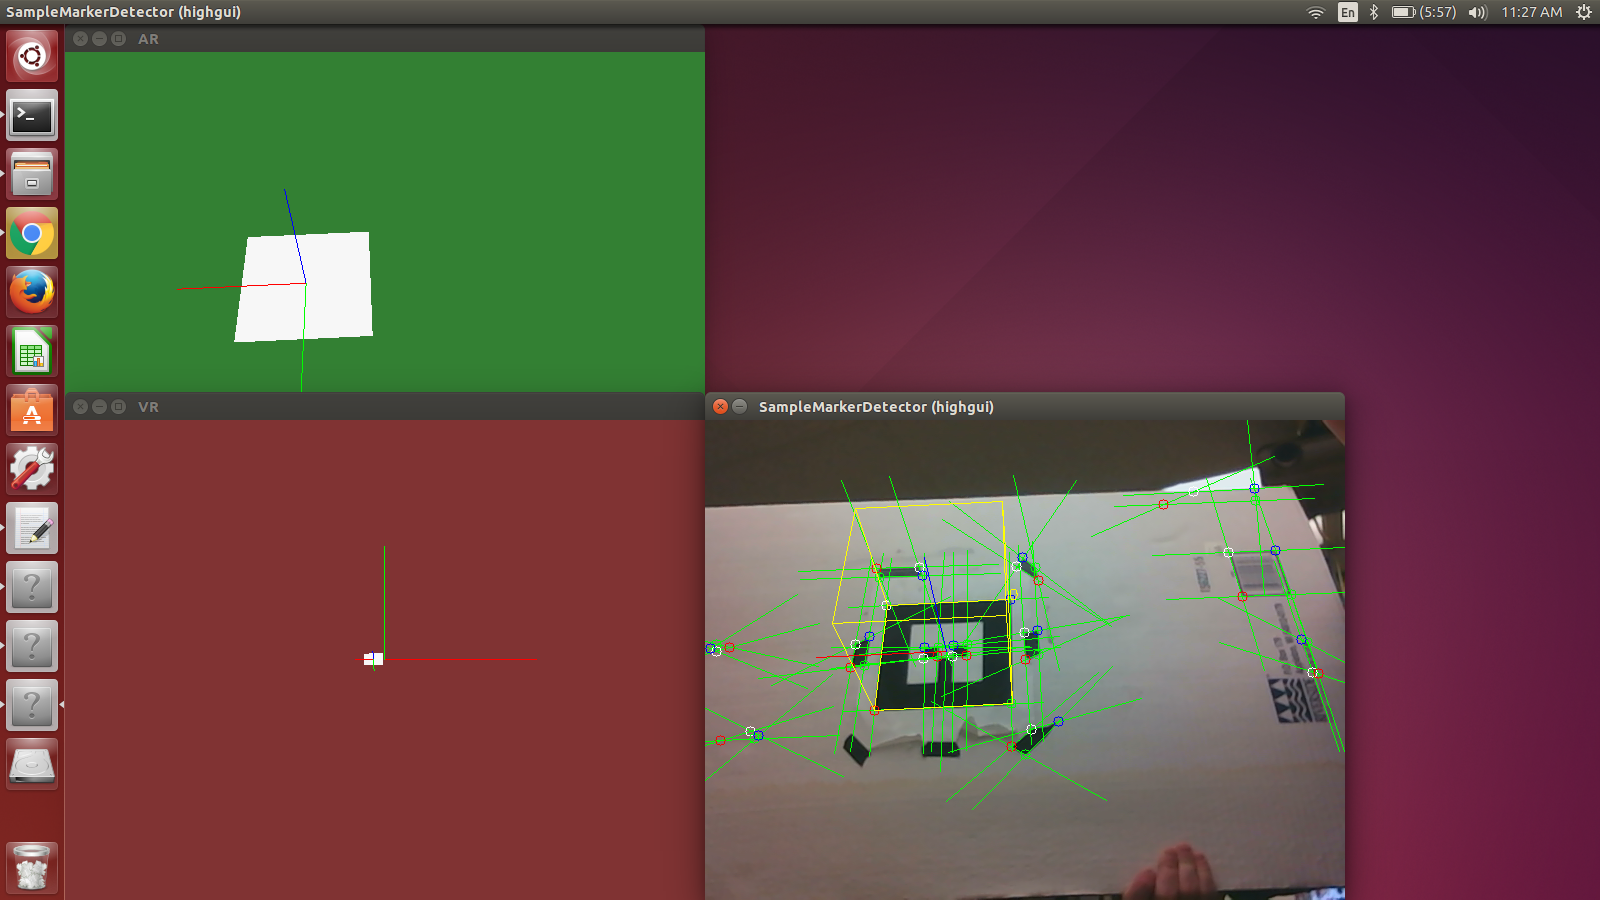
\includegraphics[width=8cm]{AlvarExample.png}
\centering
\caption{ALVAR AR Tracker testing with laptop webcam}
\label{fig:artracker}
\end{figure}

\end{itemize}


\vspace{3mm}
\noindent \large{\textbf{As an owner, I want the UAV to autonomously land on the landing pad with the correct orientation.}}
\normalsize
\begin{itemize}
\item \textbf{Landing Algorithm Simulation}\\
As mentioned previously, as our simulation development has ended, our team will utilize the sensors to generate log data to evaluate. The team will specifically test for orientation corrections that will provide the correct alignment on landing.
\item \textbf{Modify/Rewrite implementation as necessary}\\
As mentioned previously, our visual landing approach has changed. We hope to be able to easily modify the existing software to provide information regarding the orientation of the AR tag to use to change the orientation of the UAV as necessary during landing.
\end{itemize}

\vspace{6mm}
\noindent\Large{\textbf{Prototype}}\\
\normalsize
Our prototype for this sprint is mainly just an assembled hexrotor UAV that is able to follow GPS waypoints. Throughout the assembly process, we did small tests to be sure that we were on the right track. At first, we just kept the UAV in the lab and turned to rotors to verify that they were wired correctly and spinning in the right directions. We then had a manual test flight in the gym, where we discovered that the UAV is quite stable and responsive. Finally, we tested the GPS waypoint navigation with a series of flights. We started small, just having the UAV fly to the end of the driveway at first, eventually working our way up to having the UAV take off, move through a series of waypoints, and return to land on the same location it took off from. Over the course of our testing, we estimate that we will be able to trust the GPS to get us above our landing pad. As stated above, this means that we feel confident that we will be able to trust GPS to get us directly above the landing pad. \newline\newline
We have videos of these GPS tests up on \href{https://www.youtube.com/channel/UCfcuqDXKMLgbUWu3rt9rITA}{YouTube}.

